\section{TCP被动打开-服务器}
\label{sec:tcp_server_connect}
        \subsection{基本流程}
            tcp想要被动打开,就必须得先进行listen调用。而对于一台主机,它如果想要作为服务器,它会在什么时候进行listen调用呢?不难想到,它在启动某个需要TCP连接的高级应用程序的时候,就会执行listen调用。经过listen调用之后,系统内部其实创建了一个监听套接字,专门负责监听是否有数据发来,而不会负责传输数据。

            接着客户端就开始等待接收SYN段,然后回复SYN+ACK段,最后接收ACK段,三次握手建立连接。 
        \subsection{第一次握手:接受SYN段}
            \subsubsection{基本调用关系}
                \begin{figure}[htb]        
                    \centering
                    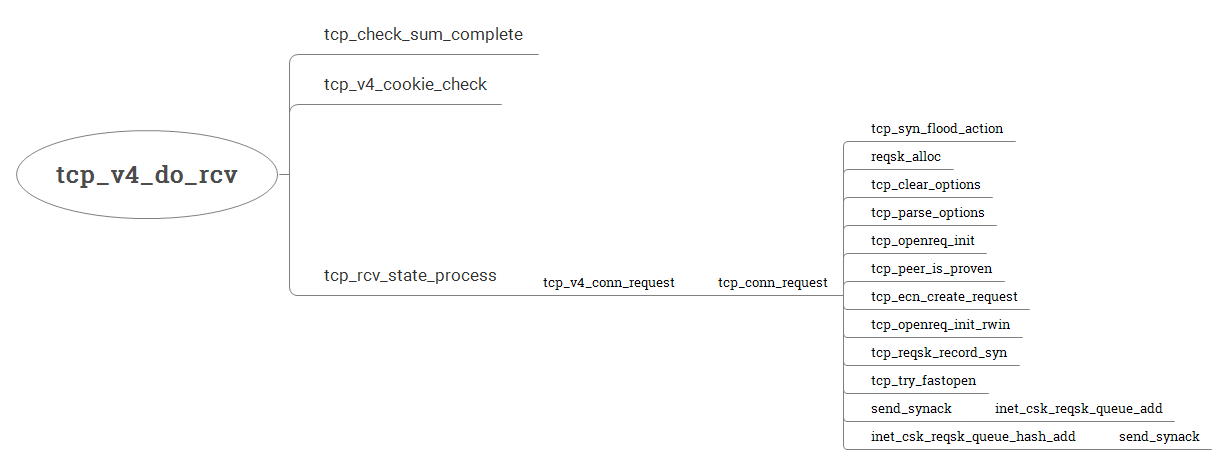
\includegraphics[width=\textwidth]{images/Server:Receive_SYN.png}
                    \caption{Server:Receive SYN}
                    \label{Server:Receive SYN}
                \end{figure}       
            \subsubsection{\mintinline{c}{tcp_v4_do_rcv}}
                \label{ServerReceiveSYN:tcp_v4_do_rcv}
                在进行第一次握手的时候,TCP必然处于LISTEN状态。传输控制块接收处理的段都由\mintinline{c}{tcp_v4_do_rcv}来处理。
\begin{minted}[linenos]{c}
/*
Location:

    net/ipv4/tcp_ipv4.c

Function:

    The socket must have it's spinlock held when we get
    here, unless it is a TCP_LISTEN socket.

    We have a potential double-lock case here, so even when
    doing backlog processing we use the BH locking scheme.
    This is because we cannot sleep with the original spinlock
    held.

Parameter:

    sk:传输控制块
    skb:传输控制块缓冲区
*/
int tcp_v4_do_rcv(struct sock *sk, struct sk_buff *skb)
{
    struct sock *rsk;

    /*省略无关代码*/
    /*基于伪首部累加和进行全包的校验和,判断包是否传输正确*/
    if (tcp_checksum_complete(skb))
        goto csum_err;
\end{minted}

        关于tcp\_checksum\_complete更多内容,请参见\ref{TCPCheckSum:tcp_checksum_complete}.

\begin{minted}[linenos]{c}
    if (sk->sk_state == TCP_LISTEN) {
        /*进行相应的cookie检查*/
        struct sock *nsk = tcp_v4_cookie_check(sk, skb);

        if (!nsk)
            goto discard;
        if (nsk != sk) {
            sock_rps_save_rxhash(nsk, skb);
            sk_mark_napi_id(nsk, skb);
            if (tcp_child_process(sk, nsk, skb)) {
                rsk = nsk;
                goto reset;
            }
            return 0;
        }
    } else
        sock_rps_save_rxhash(sk, skb);
\end{minted}
接下来处理收到的数据包,在Linux的TCP实现中,\mintinline{c}{tcp_rcv_state_process}
负责根据接收到的包维护TCP的状态机。不止是SYN段,其他收到的段大多也会交给该函数处理。
\begin{minted}[linenos]{c}
    /*处理接收到的SYN段,返回1,表示处理错误*/
    if (tcp_rcv_state_process(sk, skb)) {
        rsk = sk;
        goto reset;
    }
    return 0;

reset:
    tcp_v4_send_reset(rsk, skb);
discard:
    kfree_skb(skb);
    /* Be careful here. If this function gets more complicated and
     * gcc suffers from register pressure on the x86, sk (in \%ebx)
     * might be destroyed here. This current version compiles correctly,
     * but you have been warned.
     */
    return 0;

csum_err:
    TCP_INC_STATS_BH(sock_net(sk), TCP_MIB_CSUMERRORS);
    TCP_INC_STATS_BH(sock_net(sk), TCP_MIB_INERRS);
    goto discard;
}
\end{minted}
            
            \subsubsection{\mintinline{c}{tcp_v4_cookie_check}}
                TCP的SYN Cookie机制是为了防范SYN Flood攻击而产生的。其思想是在收到
TCP SYN包后,根据SYN包的信息计算一个cookie值作为SYN+ACK报的初始序列号。当客户端返回
ACK包时,根据返回的确认序号来判断该连接是否为一个正常的连接。
\mintinline{c}{tcp_v4_cookie_check}函数正是用于检查该cookie值的。
\begin{minted}[linenos]{c}
/*
Location

    net/ipv4/tcp_ipv4.c

Function

    cookie检查

Parameter

    sk:传输控制块
    skb:传输控制块缓冲区。  
*/
static struct sock *tcp_v4_cookie_check(struct sock *sk, struct sk_buff *skb)
{
#ifdef CONFIG_SYN_COOKIES
    const struct tcphdr *th = tcp_hdr(skb);

    if (!th->syn)
        sk = cookie_v4_check(sk, skb);
#endif
    return sk;
}
\end{minted}

                显然对于第一次握手的时候,接收到的是syn包。此时还没有cookie值,
故而直接返回了sk。
            \subsubsection{\mintinline{c}{tcp_rcv_state_process}}
                \label{Server:tcp_rcv_state_process}
                与第一次握手相关的代码如下:

\begin{minted}[linenos]{c}
/*
Location:
    
    /net/ipv4/tcp_input.c

Function:

 *  This function implements the receiving procedure of RFC 793 for
 *  all states except ESTABLISHED and TIME_WAIT.
 *  It's called from both tcp_v4_rcv and tcp_v6_rcv and should be
 *  address independent.    

Parameter

    sk:传输控制块
    skb:传输控制块缓冲区
*/

int tcp_rcv_state_process(struct sock *sk, struct sk_buff *skb)
{
    struct tcp_sock *tp = tcp_sk(sk);
    struct inet_connection_sock *icsk = inet_csk(sk);
    const struct tcphdr *th = tcp_hdr(skb);
    struct request_sock *req;
    int queued = 0;
    bool acceptable;
    /*saw_tstamp 表示在最新的包上是否看到的时间戳选项*/
    tp->rx_opt.saw_tstamp = 0;  

    switch (sk->sk_state) {
    /*省略无关代码*/

        case TCP_LISTEN:
            if (th->ack)
                return 1;

            if (th->rst)
                goto discard;

            if (th->syn) {
                if (th->fin)
                    goto discard;
                if (icsk->icsk_af_ops->conn_request(sk, skb) < 0)
                    return 1;

                /* Now we have several options: In theory there is
                 * nothing else in the frame. KA9Q has an option to
                 * send data with the syn, BSD accepts data with the
                 * syn up to the [to be] advertised window and
                 * Solaris 2.1 gives you a protocol error. For now
                 * we just ignore it, that fits the spec precisely
                 * and avoids incompatibilities. It would be nice in
                 * future to drop through and process the data.
                 *
                 * Now that TTCP is starting to be used we ought to
                 * queue this data.
                 * But, this leaves one open to an easy denial of
                 * service attack, and SYN cookies can't defend
                 * against this problem. So, we drop the data
                 * in the interest of security over speed unless
                 * it's still in use.
                 */
                kfree_skb(skb);
                return 0;
            }
            goto discard;

            /*省略无关代码*/
discard:
        __kfree_skb(skb);
    }
    return 0;
}
\end{minted}

                显然,所接收到的包的ack、rst、fin字段都不为1,故而这时开始进行连接检查,判断是否可以允许连接。经过不断查找,我们发现\mintinline{c}{icsk->icsk_af_ops->conn_request}最终会掉用\mintinline{c}{tcp_v4_conn_request}进行处理。如果syn段合法,内核就会为该连接请求创建连接请求块,并且保存相应的信息。否则,就会返回1,原函数会发送reset给客户端表明连接请求失败。

                当然,如果收到的包的ack字段为1,那么由于此时链接还未建立,故该包无效,返回1,并且调用该函数的函数会发送reset包给对方。如果收到的是rst字段或者既有fin又有syn的字段,那就直接销毁,并且释放内存。

            \subsubsection{\mintinline{c}{tcp_v4_conn_request && tcp_conn_request}}
                \label{Server:tcp_conn_request}
                该函数如下:
\begin{minted}[linenos]{c}
/* why make two functions here?
Location

    /net/ipv4/tcp_ipv4.c

Function:

    服务端用来处理客户端连接请求的函数。

Parameter:

    sk:传输控制块
    skb:传输控制块缓冲区
*/
int tcp_v4_conn_request(struct sock *sk, struct sk_buff *skb)
{
    /* Never answer to SYNs send to broadcast or multicast */
    if (skb_rtable(skb)->rt_flags & (RTCF_BROADCAST | RTCF_MULTICAST))
        goto drop;

    return tcp_conn_request(&tcp_request_sock_ops,
                &tcp_request_sock_ipv4_ops, sk, skb);

drop:
    NET_INC_STATS_BH(sock_net(sk), LINUX_MIB_LISTENDROPS);
    return 0;
}
\end{minted}
                
        如果一个SYN段是要被发送到广播地址和组播地址,则直接drop掉,然后返回0。否则的话,就继续调用\mintinline{c}{tcp_conn_request}进行连接处理。如下:

\begin{minted}[linenos]{c}
/* 
Location

    /net/ipv4/tcp_ipv4.c

Function:

    服务端用来处理客户端连接请求的函数。

Parameter:

    rsk_ops:请求控制块的函数接口
    af_ops:TCP请求块的函数接口
    sk:传输控制块
    skb:传输控制块缓冲区
*/
int tcp_conn_request(struct request_sock_ops *rsk_ops,
             const struct tcp_request_sock_ops *af_ops,
             struct sock *sk, struct sk_buff *skb)
{
    /*初始化len字段*/
    struct tcp_fastopen_cookie foc = { .len = -1 };     
    /*tw: time wait    isn: initial sequence num 初始化序列号*/
    __u32 isn = TCP_SKB_CB(skb)->tcp_tw_isn;            
    struct tcp_options_received tmp_opt;
    struct tcp_sock *tp = tcp_sk(sk);
    struct sock *fastopen_sk = NULL;
    struct dst_entry *dst = NULL;
    struct request_sock *req;
    /*标志是否开启了SYN_COOKIE选项*/
    bool want_cookie = false;
    /*路由查找相关的数据结构*/ 
    struct flowi fl;                                   

    /* TW(time wait) buckets are converted to open requests without
     * limitations, they conserve resources and peer is
     * evidently real one.
     */
    if ((sysctl_tcp_syncookies == 2 ||
         inet_csk_reqsk_queue_is_full(sk)) && !isn) {
        want_cookie = tcp_syn_flood_action(sk, skb, rsk_ops->slab_name);
        if (!want_cookie)
            goto drop;
    }
\end{minted}
                如果打开了SYNCOOKIE选项,并且SYN请求队列已满并且isn为0,然后通过函数\textbf{tcp\_syn\_flood\_action}判断是否需要发送syncookie。如果没有启用syncookie的话,就会返回false,此时不能接收新的SYN请求,会将所收到的包丢掉。

\begin{minted}[linenos]{c}
    /* Accept backlog is full. If we have already queued enough
     * of warm entries in syn queue, drop request. It is better than
     * clogging syn queue with openreqs with exponentially increasing
     * timeout.
     */
    if (sk_acceptq_is_full(sk) && inet_csk_reqsk_queue_young(sk) > 1) {
        NET_INC_STATS_BH(sock_net(sk), LINUX_MIB_LISTENOVERFLOWS);
        goto drop;
    }
\end{minted}

        如果存放已经完成连接的套接字的队列长度已经达到上限且SYN请求队列中至少有一个握手过程中没有重传过段,则丢弃当前请求。

\begin{minted}[linenos]{c}
    req = inet_reqsk_alloc(rsk_ops, sk, !want_cookie);
    if (!req)
        goto drop;
\end{minted}
            
        这时调用\mintinline{c}{inet_reqsk_alloc}分配一个连接请求块,用于保存连接请求信息,同时初始化在连接过程中用来发送ACK/RST段的操作集合,以便在建立连接过程中能方便地调用这些接口。如果申请不了资源的话,就会放弃此次连接请求。

\begin{minted}[linenos]{c}
    tcp_rsk(req)->af_specific = af_ops;
    tcp_clear_options(&tmp_opt);
    tmp_opt.mss_clamp = af_ops->mss_clamp;
    tmp_opt.user_mss  = tp->rx_opt.user_mss;
    tcp_parse_options(skb, &tmp_opt, 0, want_cookie ? NULL : &foc);
\end{minted}

        之后,清除TCP选项,初始化\mintinline{c}{mss_vlamp}和\mintinline{c}{user_mss}.然后调用\mintinline{c}{tcp_parse_options}解析SYN段中的TCP选项,查看是否有相关的选项。

        关于tcp\_clear\_options的更多内容,请参见\ref{TCPOptions:tcp_clear_options}。
\begin{minted}[linenos]{c}
    if (want_cookie && !tmp_opt.saw_tstamp)
        tcp_clear_options(&tmp_opt);
\end{minted}

        如果启动了syncookies,并且TCP选项中没有存在时间戳,则清除已经解析的TCP选项。这是因为计算\mintinline{c}{syn_cookie}必须用到时间戳。

\begin{minted}[linenos]{c}
    /* tstamp_ok表示在收到的SYN包上看到的TIMESTAMP*/
    tmp_opt.tstamp_ok = tmp_opt.saw_tstamp;        
    tcp_openreq_init(req, &tmp_opt, skb, sk);
\end{minted}

        这时,根据收到的SYN段中的选项和序号来初始化连接请求块信息。

\begin{minted}[linenos]{c}
    /* Note: tcp_v6_init_req() might override ir_iif for link locals */
    inet_rsk(req)->ir_iif = sk->sk_bound_dev_if;

    af_ops->init_req(req, sk, skb);

    if (security_inet_conn_request(sk, skb, req))
        goto drop_and_free;
\end{minted}

        这一部分于IPV6以及安全检测有关,这里不进行详细讲解。安全检测失败的话,就会丢弃SYN段。

\begin{minted}[linenos]{c}
    if (!want_cookie && !isn) {
        /* VJ's idea. We save last timestamp seen
         * from the destination in peer table, when entering
         * state TIME-WAIT, and check against it before
         * accepting new connection request.
         *
         * If "isn" is not zero, this request hit alive
         * timewait bucket, so that all the necessary checks
         * are made in the function processing timewait state.
         */
        if (tcp_death_row.sysctl_tw_recycle) {
            bool strict;

            dst = af_ops->route_req(sk, &fl, req, &strict);

            if (dst && strict &&
                !tcp_peer_is_proven(req, dst, true,
                        tmp_opt.saw_tstamp)) {
                NET_INC_STATS_BH(sock_net(sk), LINUX_MIB_PAWSPASSIVEREJECTED);
                goto drop_and_release;
            }
        }
        /* Kill the following clause, if you dislike this way. */
        else if (!sysctl_tcp_syncookies &&
             (sysctl_max_syn_backlog - inet_csk_reqsk_queue_len(sk) <
              (sysctl_max_syn_backlog >> 2)) &&
             !tcp_peer_is_proven(req, dst, false,
                         tmp_opt.saw_tstamp)) {
            /* Without syncookies last quarter of
             * backlog is filled with destinations,
             * proven to be alive.
             * It means that we continue to communicate
             * to destinations, already remembered
             * to the moment of synflood.
             */
            pr_drop_req(req, ntohs(tcp_hdr(skb)->source),
                    rsk_ops->family);
            goto drop_and_release;
        }

        isn = af_ops->init_seq(skb);
    }
\end{minted}

        如果没有开启syncookie并且isn为0的话,其中的第一个if从对段信息块中获取时间戳,在新的连接请求之前检测\textbf{PAWS}。后边的表明在没有启动syncookies的情况下受到synflood攻击,丢弃收到的段。之后由源地址,源端口,目的地址以及目的端口计算出服务端初始序列号。

\begin{minted}[linenos]{c}
    if (!dst) {
        dst = af_ops->route_req(sk, &fl, req, NULL);
        if (!dst)
            goto drop_and_free;
    }
    /*显示拥塞控制*/
    tcp_ecn_create_request(req, skb, sk, dst);

    /*如果开启了cookie的话,就需要进行相应的初始化*/
    if (want_cookie) {
        isn = cookie_init_sequence(af_ops, sk, skb, &req->mss);
        req->cookie_ts = tmp_opt.tstamp_ok;
        if (!tmp_opt.tstamp_ok)
            inet_rsk(req)->ecn_ok = 0;
    }

    tcp_rsk(req)->snt_isn = isn;
    tcp_rsk(req)->txhash = net_tx_rndhash();
    tcp_openreq_init_rwin(req, sk, dst);
    if (!want_cookie) {
        tcp_reqsk_record_syn(sk, req, skb);
        fastopen_sk = tcp_try_fastopen(sk, skb, req, &foc, dst);
    }

    /*如果开启了fastopen的话,顺便发送数据
        否则就是简单地发送。
    */
    if (fastopen_sk) {
        af_ops->send_synack(fastopen_sk, dst, &fl, req,
                    &foc, false);
        /* Add the child socket directly into the accept queue */
        inet_csk_reqsk_queue_add(sk, req, fastopen_sk);
        sk->sk_data_ready(sk);
        bh_unlock_sock(fastopen_sk);
        sock_put(fastopen_sk);
    } else {
        tcp_rsk(req)->tfo_listener = false;
        if (!want_cookie)
            inet_csk_reqsk_queue_hash_add(sk, req, TCP_TIMEOUT_INIT);
        af_ops->send_synack(sk, dst, &fl, req,
                    &foc, !want_cookie);
        if (want_cookie)
            goto drop_and_free;
    }
    reqsk_put(req);
    return 0;

drop_and_release:
    dst_release(dst);
drop_and_free:
    reqsk_free(req);
drop:
    NET_INC_STATS_BH(sock_net(sk), LINUX_MIB_LISTENDROPS);
    return 0;
\end{minted}

            关于\mintinline{c}{inet_csk_reqsk_queue_add}的更多内容请参见\ref{INET:inet_csk_reqsk_queue_add}。
            关于\mintinline{c}{inet_csk_reqsk_queue_hash_add}的更多的内容请参见\ref{INET:inet_csk_reqsk_queue_hash_add}。

%----------------------------------------------------------------------------------------
%                   Server:     Send    SYN+ACK
%----------------------------------------------------------------------------------------

        \subsection{第二次握手:发送SYN+ACK段}
            在第一次握手的最后调用了\mintinline{c}{af_ops->send_synack}函数,而该函数最终会调用\mintinline{c}{tcp_v4_send_synack}函数进行发送,故而这里我们这里就从这个函数进行分析。
            \subsubsection{基本调用关系}            
                \begin{figure}[htb]        
                   \center{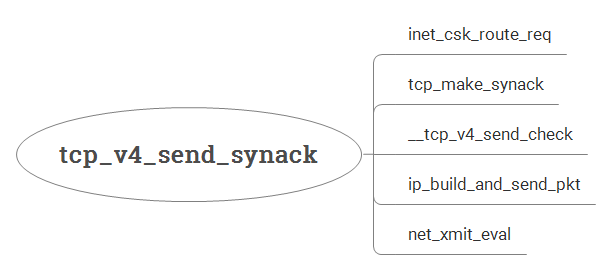
\includegraphics[width=\textwidth]{images/Server:Send_SYN+ACK.png}}
                    \caption{Server:Send SYN+ACK}
                    \label{Server:Send SYN+ACK}
                \end{figure}   
            \subsubsection{tcp\_v4\_send\_synack}
                \label{ServerSendSYN+ACK:tcp_v4_send_synack}
\begin{minted}[linenos]{c}
/*
Location:

    net/ipv4/tcp_ipv4.c

Function: 

    Send a SYN-ACK after having received a SYN.
    This still operates on a request_sock only, not on a big
    socket.

Paramaters:

    sk:传输控制块
    dst:存储缓存路由项中独立于协议的信息。
    fl:
    req:请求控制块
    foc:快打开缓存
    attach_req:

*/
static int tcp_v4_send_synack(const struct sock *sk, struct dst_entry *dst,
                  struct flowi *fl,
                  struct request_sock *req,
                  struct tcp_fastopen_cookie *foc,
                  bool attach_req)
{
    const struct inet_request_sock *ireq = inet_rsk(req);
    struct flowi4 fl4;
    int err = -1;
    struct sk_buff *skb;

    /* First, grab a route. */
    if (!dst && (dst = inet_csk_route_req(sk, &fl4, req)) == NULL)
        return -1;
\end{minted}

    首先,如果传进来的dst为空或者根据连接请求块中的信息查询路由表,如果没有查到,那么就直接退出。       

\begin{minted}[linenos]{c}
    /*根据当前的传输控制块,路由信息,请求等信息构建syn+ack段*/
    skb = tcp_make_synack(sk, dst, req, foc, attach_req);
    /*
        如果构建成功的话,就生成TCP校验码,然后调用
        ip_build_and_send_pkt生成IP数据报并且发送出去。
    */
    if (skb) {
        __tcp_v4_send_check(skb, ireq->ir_loc_addr, ireq->ir_rmt_addr);

        err = ip_build_and_send_pkt(skb, sk, ireq->ir_loc_addr,
                        ireq->ir_rmt_addr,
                        ireq->opt);
        err = net_xmit_eval(err);
    }
    return err;
}
\end{minted}
                \mintinline{c}{net_xmit_eval}用于过滤错误码中的拥塞提示错误,换句
话说,就是如果错误是由于拥塞造成的,那么就忽略掉,否则就返回错误码。
            \subsubsection{\mintinline{c}{tcp_make_synack}}
                \label{ServerSendSYN+ACK:tcp_make_synack}

\begin{minted}[linenos]{c}
/*
Location:

    net/ipv4/ycp_output.c

Function:
        tcp_make_synack - Prepare a SYN-ACK.
        Allocate one skb and build a SYNACK packet.
        @dst is consumed : Caller should not use it again.

        该函数用来构造一个SYN+ACK段,
        并初始化TCP首部及SKB中的各字段项,
        填入相应的选项,如MSS,SACK,窗口扩大因子,时间戳等。

Parameter:
        sk          : listener socket
        dst         : dst entry attached to the SYNACK
        req         : request_sock pointer
        foc         : fast open cookie
        attach_req  :
 */
struct sk_buff *tcp_make_synack(const struct sock *sk, struct dst_entry *dst,
                struct request_sock *req,
                struct tcp_fastopen_cookie *foc,
                bool attach_req)
{
    struct inet_request_sock *ireq = inet_rsk(req);
    const struct tcp_sock *tp = tcp_sk(sk);
    struct tcp_md5sig_key *md5 = NULL;
    struct tcp_out_options opts;
    struct sk_buff *skb;
    int tcp_header_size;
    struct tcphdr *th;
    u16 user_mss;
    int mss;

    skb = alloc_skb(MAX_TCP_HEADER, GFP_ATOMIC);
    if (unlikely(!skb)) {
        dst_release(dst);
        return NULL;
    }
\end{minted}

    首先为将要发送的数据申请发送缓存,如果没有申请到,那就会返回NULL。

    关于unlikely优化的更多内容,请参见\ref{GCC:likely && unlikely}.

\begin{minted}[linenos]{c}
    /* Reserve space for headers. */
    skb_reserve(skb, MAX_TCP_HEADER);
\end{minted}

    为MAC层,IP层,TCP层首部预留必要的空间。

\begin{minted}[linenos]{c}
    if (attach_req) {
        skb_set_owner_w(skb, req_to_sk(req));
    } else {
        /* sk is a const pointer, because we want to express multiple
         * cpu might call us concurrently.
         * sk->sk_wmem_alloc in an atomic, we can promote to rw.
         */
        skb_set_owner_w(skb, (struct sock *)sk);
    }
    skb_dst_set(skb, dst);
\end{minted}

    根据\mintinline{c}{attach_req}来判断该执行如何执行相关操作。然后设置发送缓存的
目的路由。%TODO: what is attach_req means?

\begin{minted}[linenos]{c}
    mss = dst_metric_advmss(dst);
    user_mss = READ_ONCE(tp->rx_opt.user_mss);
    if (user_mss && user_mss < mss)
        mss = user_mss;
\end{minted}

    根据每一个路由器上的mss以及自身的mss来得到最大的mss。

\begin{minted}[linenos]{c}
    memset(&opts, 0, sizeof(opts));
#ifdef CONFIG_SYN_COOKIES
    if (unlikely(req->cookie_ts))
        skb->skb_mstamp.stamp_jiffies = cookie_init_timestamp(req);
    else
#endif
    skb_mstamp_get(&skb->skb_mstamp);
\end{minted}

    清除选项,并且设置相关时间戳。

\begin{minted}[linenos]{c}
#ifdef CONFIG_TCP_MD5SIG
    rcu_read_lock();
    md5 = tcp_rsk(req)->af_specific->req_md5_lookup(sk, req_to_sk(req));
#endif
\end{minted}

    查看是否有MD5选项,有的话构造出相应的md5.

\begin{minted}[linenos]{c}
    skb_set_hash(skb, tcp_rsk(req)->txhash, PKT_HASH_TYPE_L4);
    tcp_header_size = tcp_synack_options(req, mss, skb, &opts, md5, foc) +
              sizeof(*th);

    skb_push(skb, tcp_header_size);
    skb_reset_transport_header(skb);
\end{minted}

    得到tcp的头部大小,然后进行大小设置,并且重置传输层的头部。

\begin{minted}[linenos]{c}
    th = tcp_hdr(skb);
    memset(th, 0, sizeof(struct tcphdr));
    th->syn = 1;
    th->ack = 1;
    tcp_ecn_make_synack(req, th);
    th->source = htons(ireq->ir_num);
    th->dest = ireq->ir_rmt_port;
\end{minted}

    清空tcp头部,并设置tcp头部的各个字段。

\begin{minted}[linenos]{c}
    /* Setting of flags are superfluous here for callers (and ECE is
     * not even correctly set)
     */
    tcp_init_nondata_skb(skb, tcp_rsk(req)->snt_isn,
                 TCPHDR_SYN | TCPHDR_ACK);

    th->seq = htonl(TCP_SKB_CB(skb)->seq);
    /* XXX data is queued and acked as is. No buffer/window check */
    th->ack_seq = htonl(tcp_rsk(req)->rcv_nxt);

    /* RFC1323: The window in SYN & SYN/ACK segments is never scaled. */
    th->window = htons(min(req->rsk_rcv_wnd, 65535U));
    tcp_options_write((__be32 *)(th + 1), NULL, &opts);
    th->doff = (tcp_header_size >> 2);
    TCP_INC_STATS_BH(sock_net(sk), TCP_MIB_OUTSEGS);
\end{minted}

    首先初始化不含数据的tcp报文,然后设置相关的序列号,确认序列号,窗口大小,选项字段,以及TCP数据偏移,之所以除以4,是doff的单位是32位字,即以四个字节长的字为计算单位。
           
    关于tcp\_init\_nondata\_skb更多的内容,请参见\ref{TCPInitialize:tcp_init_nondata_skb}。
     
\begin{minted}[linenos]{c}
#ifdef CONFIG_TCP_MD5SIG
    /* Okay, we have all we need - do the md5 hash if needed */
    if (md5)
        tcp_rsk(req)->af_specific->calc_md5_hash(opts.hash_location,
                           md5, req_to_sk(req), skb);
    rcu_read_unlock();
#endif

    /* Do not fool tcpdump (if any), clean our debris */
    skb->tstamp.tv64 = 0;
    return skb;
}
\end{minted}

    最后判断是否需要md5哈希值,如果需要的话,就进行添加。最后返回生成包含SYN+ACK段的skb。  

        \subsection{第三次握手:接收ACK段}

            在服务器第二次握手的最后启动了建立连接定时器,等待客户端最后一次握手的ACK段。           
            \subsubsection{基本调用关系}
                \begin{figure}[htb]        
                    \center{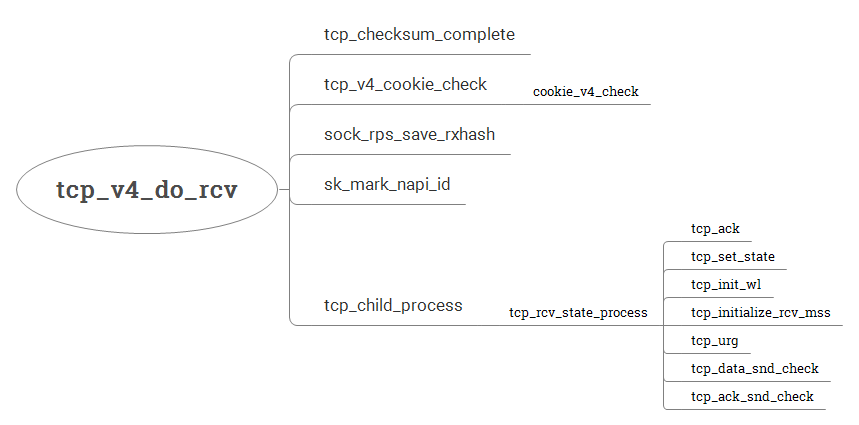
\includegraphics[width=\textwidth]{images/Server:Receive_ACK.png}}
                    \caption{Server:Receive ACK}
                    \label{Server:Receive ACK}
                \end{figure}  
            \subsubsection{\mintinline{c}{tcp_v4_do_rcv}}
                \label{ServerReceiveACK:tcp_v4_do_rcv}
\begin{minted}[linenos]{c}
/* 
Location:

    /net/ipv4/tcp_ipv4.c

Function:

    The socket must have it's spinlock held when we get
    here, unless it is a TCP_LISTEN socket.

    We have a potential double-lock case here, so even when
    doing backlog processing we use the BH locking scheme.
    This is because we cannot sleep with the original spinlock
    held.

Parameter:

    sk:传输控制块。
    skb:传输控制块缓冲区。
*/
int tcp_v4_do_rcv(struct sock *sk, struct sk_buff *skb)
{
    struct sock *rsk;

    /**省略无关代码**/

    if (tcp_checksum_complete(skb))
        goto csum_err;

    if (sk->sk_state == TCP_LISTEN) {
        /*
            NULL,错误 
            nsk == sk,接收到SYN 
            nsk != sk,接收到ACK 
        */
        struct sock *nsk = tcp_v4_cookie_check(sk, skb);

        if (!nsk)
            goto discard;
        if (nsk != sk) {
            sock_rps_save_rxhash(nsk, skb);
            sk_mark_napi_id(nsk, skb);
            if (tcp_child_process(sk, nsk, skb)) {
                rsk = nsk;
                goto reset;
            }
            return 0;
        }
    } else
        sock_rps_save_rxhash(sk, skb);
    /**省略无关代码**/
reset:
    tcp_v4_send_reset(rsk, skb);
discard:
    kfree_skb(skb);
    /* Be careful here. If this function gets more complicated and
     * gcc suffers from register pressure on the x86, sk (in %ebx)
     * might be destroyed here. This current version compiles correctly,
     * but you have been warned.
     */
    return 0;

csum_err:
    TCP_INC_STATS_BH(sock_net(sk), TCP_MIB_CSUMERRORS);
    TCP_INC_STATS_BH(sock_net(sk), TCP_MIB_INERRS);
    goto discard;
}
\end{minted}
                    在服务器最后一次握手的时候,其实传输控制块仍然处于LISTEN状态,但是这时候cookie检查得到的传输控制块已经不是侦听传输控制块了,故而会执行\mintinline{c}{tcp_child_process}来初始化子传输控制块。如果初始化失败的话(返回值非零),就会给客户端发送RST段进行复位。

                \subsubsection{\mintinline{c}{tcp_v4_cookie_check}}

\begin{minted}[linenos]{c}
static struct sock *tcp_v4_cookie_check(struct sock *sk, struct sk_buff *skb)
{
#ifdef CONFIG_SYN_COOKIES
    const struct tcphdr *th = tcp_hdr(skb);

    if (!th->syn)
        sk = cookie_v4_check(sk, skb);
#endif
    return sk;
}
\end{minted}

                   如果Linux内核中定义\mintinline{c}{CONFIG_SYN_COOKIES}宏,此时在第三次握手阶段,并不是syn包,内核就会执行\mintinline{c}{cookie_v4_check}。在这个函数中,服务器会将客户端的ACK序列号减去1,得到cookie比较值,然后将客户端的IP地址,客户端端口,服务器IP地址和服务器端口,接收到的TCP序列好以及其它一些安全数值等要素进行hash运算后,与该cookie比较值比较,如果相等,则直接完成三次握手,此时不必查看该连接是否属于请求连接队列。

                \subsubsection{\mintinline{c}{tcp_child_process}}

                    该函数位于\mintinline{c}{/net/ipv4/minisocks.c}中,子传输控制块开始处理TCP段。

\begin{minted}[linenos]{c}
/*
Location:

    net/ipv4/tcp_minisock.c

Functions:

    Queue segment on the new socket if the new socket is active,
    otherwise we just shortcircuit this and continue with
    the new socket.

    For the vast majority of cases child->sk_state will be TCP_SYN_RECV
    when entering. But other states are possible due to a race condition
    where after __inet_lookup_established() fails but before the listener
    locked is obtained, other packets cause the same connection to
    be created.
Parameters:

    parent:父传出控制块
    child:子传输控制块
    skb:传输控制块缓存
*/

int tcp_child_process(struct sock *parent, struct sock *child,
              struct sk_buff *skb)
{
    int ret = 0;
    int state = child->sk_state;

    tcp_sk(child)->segs_in += max_t(u16, 1, skb_shinfo(skb)->gso_segs);
    if (!sock_owned_by_user(child)) {
        ret = tcp_rcv_state_process(child, skb);
        /* Wakeup parent, send SIGIO */
        if (state == TCP_SYN_RECV && child->sk_state != state)
            parent->sk_data_ready(parent);
    } else {
        /* Alas, it is possible again, because we do lookup
         * in main socket hash table and lock on listening
         * socket does not protect us more.
         */
        __sk_add_backlog(child, skb);
    }

    bh_unlock_sock(child);
    sock_put(child);
    return ret;
}
\end{minted}

                首先,如果此时刚刚创建的新的子传输控制块没有被用户进程占用,则根据第三次握手的ACK段,调用\mintinline{c}{tcp_rcv_state_process}继续对子传输控制块做初始化。否则的话,只能将其加入后备队列中,等空闲时再进行处理。虽然这种情况出现的概率小,但是也是有可能发生的。

        \subsubsection{\mintinline{c}{tcp_rcv_state_process}}

            该函数位于\mintinline{c}{/net/ipv4/tcp_input.c}中。
            
            该函数用来处理ESTABLISHED和\mintinline{c}{TIME_WAIT}状态以外的TCP段,这里处理\mintinline{c}{SYN_RECV}状态。

\begin{minted}[linenos]{c}
    acceptable = tcp_ack(sk, skb, FLAG_SLOWPATH |
                      FLAG_UPDATE_TS_RECENT) > 0;
\end{minted}

    首先对收到的ACK段进行处理判断是否正确接收,如果正确接收就会发送返回非零值。

\begin{minted}[linenos]{c}
    switch (sk->sk_state) {
        case TCP_SYN_RECV:
            if (!acceptable)
                return 1;

            if (!tp->srtt_us)
                tcp_synack_rtt_meas(sk, req);

            /* Once we leave TCP_SYN_RECV, we no longer need req
             * so release it.
             */
            if (req) {
                tp->total_retrans = req->num_retrans;
                reqsk_fastopen_remove(sk, req, false);
            } else {
                /* Make sure socket is routed, for correct metrics. */
                icsk->icsk_af_ops->rebuild_header(sk);
                tcp_init_congestion_control(sk);

                tcp_mtup_init(sk);
                tp->copied_seq = tp->rcv_nxt;
                tcp_init_buffer_space(sk);
            }
            smp_mb();
            tcp_set_state(sk, TCP_ESTABLISHED);
            sk->sk_state_change(sk);
\end{minted}

    进行一系列的初始化,开启相应拥塞控制等,并且将TCP的状态置为ESTABLISHED。

\begin{minted}[linenos]{c}

            /* Note, that this wakeup is only for marginal crossed SYN case.
             * Passively open sockets are not waked up, because
             * sk->sk_sleep == NULL and sk->sk_socket == NULL.
             */
            if (sk->sk_socket)
                sk_wake_async(sk, SOCK_WAKE_IO, POLL_OUT);
\end{minted}

    发信号给那些将通过该套接口发送数据的进程,通知它们套接口目前已经可以发送数据了。

\begin{minted}[linenos]{c}
            tp->snd_una = TCP_SKB_CB(skb)->ack_seq;
            tp->snd_wnd = ntohs(th->window) << tp->rx_opt.snd_wscale;
            tcp_init_wl(tp, TCP_SKB_CB(skb)->seq);

            if (tp->rx_opt.tstamp_ok)
                tp->advmss -= TCPOLEN_TSTAMP_ALIGNED;
\end{minted}

    初始化传输控制块的各个字段,对时间戳进行处理。

\begin{minted}[linenos]{c}
            if (req) {
                /* Re-arm the timer because data may have been sent out.
                 * This is similar to the regular data transmission case
                 * when new data has just been ack'ed.
                 *
                 * (TFO) - we could try to be more aggressive and
                 * retransmitting any data sooner based on when they
                 * are sent out.
                 */
                tcp_rearm_rto(sk);
            } else
                tcp_init_metrics(sk);
\end{minted}

    为该套接口初始化路由。

\begin{minted}[linenos]{c}
            tcp_update_pacing_rate(sk);

            /* Prevent spurious tcp_cwnd_restart() on first data packet */
            tp->lsndtime = tcp_time_stamp;

            tcp_initialize_rcv_mss(sk);
            tcp_fast_path_on(tp);
            break;
\end{minted}

    更新最近一次的发送数据报的时间,初始化与路径MTU有关的成员,并计算有关TCP首部预测的标志。

\begin{minted}[linenos]{c}
    /* step 6: check the URG bit */
    tcp_urg(sk, skb, th);
\end{minted}

    检测带外数据标志位。

    关于tcp\_urg的详细内容,请参见\ref{TCPUrgent:tcp_urg}.

\begin{minted}[linenos]{c}
    /* step 7: process the segment text */
    switch (sk->sk_state) {
        /**省略无关代码**/
        case TCP_ESTABLISHED:
            tcp_data_queue(sk, skb);
            queued = 1;
            break;
    }
\end{minted}

                对已接收到的TCP段排队,在建立连接阶段一般不会收到TCP段。

\begin{minted}[linenos]{c}
    /* tcp_data could move socket to TIME-WAIT */
    if (sk->sk_state != TCP_CLOSE) {
        tcp_data_snd_check(sk);
        tcp_ack_snd_check(sk);
    }

    if (!queued) {
discard:
        __kfree_skb(skb);
    }
    return 0;
\end{minted}

                显然此时状态不为CLOSE,故而就回去检测是否数据和ACK要发送。其次,根据queue标志来确定是否释放接收到的TCP段,如果接收到的TCP段已添加到接收队列中,则不释放。
